\chapter{Extreme Values and the L Functions of Eta Products}\label{ch:11}

Euler's pentagonal number theorem expands $\prod_{n\ge1}(1-q^n)$ as a lacunary series, and Jacobi's triple product does the same for theta functions. A probabilist reads these products differently. A product of numbers in $(0,1)$ is the probability that independent events all occur, and $1-e^{-\lambda y}$ is the probability that an exponential clock of rate $\lambda$ has rung by time $y$. So $\prod_n(1-e^{-2\pi ny})$ is the probability that every clock in an infinite family has rung by time $y$: it is the distribution function of a maximum. This leads to a representation, new in this book, of the $L$ function of Ramanujan's $\Delta$, and of every multiplicative eta product, as the expectation of a regularised incomplete gamma function at an extreme value. For real $s>0$ it is a probability, so $L(E_{11a},1)$, an Artin $L$ value, Catalan's constant and $\pi/4$ become probabilities that a gamma variable beats a maximum of exponentials. Modularity becomes self similarity of a law, and we obtain a Monte Carlo method. The representation does not locate the nontrivial zeros, and we explain why.

\section{The product as a distribution function}

Let $E_1,E_2,\ldots$ be independent standard exponential variables and set
\[
M=\max_{n\ge1}\frac{E_n}{2\pi n},\qquad P(y)=\prod_{n\ge1}\bigl(1-e^{-2\pi ny}\bigr)\quad(y>0).
\]
The Dedekind eta function\index{Dedekind eta function} is $\eta(\tau)=q^{1/24}\prod_{n\ge1}(1-q^n)$ with $q=e^{2\pi i\tau}$, so that $\eta(iy)=e^{-\pi y/12}P(y)$.

\begin{proposition}[this book]\label{prop:ch11M}
The variable $M$ is almost surely finite and positive, and $\Prob(M\le y)=P(y)$ for $y>0$. The function $P$ is continuous and strictly increasing, and
\[
1-P(y)\sim e^{-2\pi y}\quad(y\to\infty),\qquad P(y)\sim y^{-1/2}e^{-\pi/(12y)}\quad(y\to0).
\]
The density of $M$ is $\tfrac{2\pi}{24}\bigl(1-E_2(iy)\bigr)P(y)$, where $E_2=1-24\sum_{N\ge1}\sigma(N)q^N$ is the quasimodular Eisenstein series of weight two.
\end{proposition}

\begin{proof}
Fix $y>0$. The events $A_n=\{E_n\le2\pi ny\}$ are independent with $\Prob(A_n)=1-e^{-2\pi ny}$, and $\{M\le y\}=\bigcap_nA_n$. By continuity along the decreasing events $\bigcap_{n\le N}A_n$, $\Prob(M\le y)=\lim_N\prod_{n\le N}(1-e^{-2\pi ny})$. Since $\sum_ne^{-2\pi ny}<\infty$ the product converges to a positive limit, which is $P(y)$, and $\prod(1-x_n)\ge1-\sum x_n$ gives
\[
1-\frac{e^{-2\pi y}}{1-e^{-2\pi y}}\le P(y)\le1-e^{-2\pi y}.
\]
This yields the right tail and $M<\infty$ almost surely. Uniform convergence of $\sum_n\log(1-e^{-2\pi ny})$ on $[a,\infty)$ for each $a>0$ gives continuity, and each factor is strictly increasing. Differentiating the logarithm termwise,
\[
\frac{P'(y)}{P(y)}=\sum_{n\ge1}\frac{2\pi n\,e^{-2\pi ny}}{1-e^{-2\pi ny}}=2\pi\sum_{N\ge1}\sigma(N)e^{-2\pi Ny}=\frac{2\pi}{24}\bigl(1-E_2(iy)\bigr).
\]
For small $y$ we use $\eta(-1/\tau)=\sqrt{\tau/i}\,\eta(\tau)$, which at $\tau=iy$ reads $\eta(i/y)=\sqrt y\,\eta(iy)$. Inserting $\eta(iy)=e^{-\pi y/12}P(y)$ on both sides gives
\begin{equation}\label{eq:ch11Pmod}
P(y)=y^{-1/2}\,e^{\pi y/12-\pi/(12y)}\,P(1/y).
\end{equation}
As $y\to0$, $P(1/y)\to1$, so $P(y)\sim y^{-1/2}e^{-\pi/(12y)}$; in particular $M>0$ almost surely.
\end{proof}

The right tail is that of the first clock alone. The left tail decays like $e^{-\pi/(12y)}$, so $\E[M^{-a}]<\infty$ for every $a>0$, and this is what will make our representations valid on the whole complex plane. The mean has a closed form, $\E[M]=2/\sqrt3-3/\pi=0.1997709\ldots$ (Exercise~\ref{ex:ch11mean}).

\subsection{Gumbel behaviour and the R\'enyi representation}

Because $1-P(y)\sim e^{-2\pi y}$, the law of $M$ lies in the Gumbel domain of attraction\index{Gumbel law} \cite{fishertippett1928,gnedenko1943}: $P\bigl((z+\log m)/(2\pi)\bigr)^m\to e^{-e^{-z}}$ as $m\to\infty$, and at $z=0$ the left side is $0.34475$, $0.36235$, $0.36733$ for $m=24,100,1000$, against $e^{-1}=0.36788$. R\'enyi's representation \cite{renyi1953}\index{R\'enyi representation} writes the maximum of $m$ independent standard exponentials, in law, as $\sum_{j\le m}E'_j/j$ with $E'_j$ independent standard exponentials, a generalized gamma convolution with Thorin measure $\sum_{j\le m}\delta_j$ (Chapter~\ref{ch:10}). Our $M$ has \emph{different} rates $2\pi n$, and it is not a sum of independent exponential variables at all (Exercise~\ref{ex:ch11laplace}); in exchange, the arithmetic of the rates makes $P$ modular.

\section{Ramanujan's Delta as an extreme value law}

Let $E_{j,n}$ ($j\le24$, $n\ge1$) be independent standard exponentials and
\[
M^*=\max_{j\le24,\,n\ge1}\frac{E_{j,n}}{2\pi n},\qquad F(y)=\Prob(M^*\le y)=P(y)^{24},
\]
so that $M^*$ is the maximum of $24$ independent copies of $M$. Since $\Delta=\eta^{24}=q\prod_n(1-q^n)^{24}$,
\begin{equation}\label{eq:ch11DeltaF}
\Delta(iy)=e^{-2\pi y}F(y)\qquad(y>0).
\end{equation}
Figure~\ref{fig:mstar} shows $F$ and its density.\index{extreme value representation}

\begin{figure}[t]
\centering
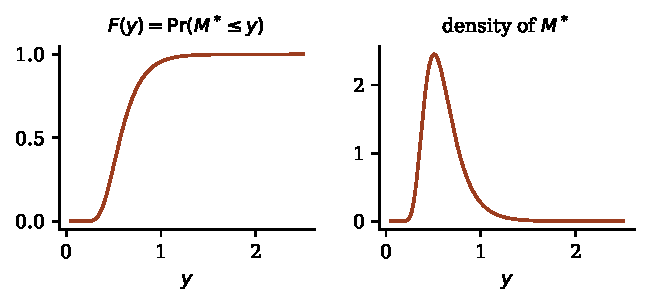
\includegraphics[width=\textwidth]{figs/mstar.pdf}
\caption{The distribution function $F(y)=\prod_n(1-e^{-2\pi ny})^{24}$ of $M^*=\max_{j\le24,\,n\ge1}E_{j,n}/(2\pi n)$, with $E_{j,n}$ independent standard exponential variables (left), and its density (right). The function $e^{-2\pi y}F(y)$ is $\Delta(iy)$.}
\label{fig:mstar}
\end{figure}

For complex $s$ and $c>0$ let $Q(s,c)=\Gamma(s,c)/\Gamma(s)$ be the regularised upper incomplete gamma function,\index{incomplete gamma function}
\[
Q(s,c)=\frac1{\Gamma(s)}\int_c^\infty t^{s-1}e^{-t}\,dt .
\]
For fixed $c>0$, $\Gamma(\cdot,c)$ and $1/\Gamma$ are entire, so $Q(\cdot,c)$ is entire and vanishes at $s=0,-1,-2,\ldots$. For real $s>0$, $Q(s,c)=\Prob(G_s\ge c)$, where $G_s$ has the gamma law of shape $s$ and unit rate.

\begin{theorem}[this book]\label{thm:ch11main}
For every complex $s$,
\[
L(s,\Delta)=\E\bigl[Q(s,2\pi M^*)\bigr].
\]
For real $s>0$, equivalently, $L(s,\Delta)=\Prob(G_s\ge2\pi M^*)$ with $G_s$ independent of $M^*$.
\end{theorem}

\begin{proof}
Recall from Chapter~\ref{ch:02} that for $\operatorname{Re}s>7$ the Dirichlet series converges absolutely and, by termwise integration,
\[
\Lambda(s,\Delta)=(2\pi)^{-s}\Gamma(s)L(s,\Delta)=\int_0^\infty\Delta(iy)y^{s-1}dy.
\]

\emph{Step 1.} By~\eqref{eq:ch11DeltaF}, $0<\Delta(iy)\le e^{-2\pi y}$, and modularity gives $\Delta(iy)=y^{-12}\Delta(i/y)$, which is at most $y^{-12}e^{-2\pi/y}$. Hence $\int_0^\infty\Delta(iy)y^{\sigma-1}dy<\infty$ for every real $\sigma$, locally uniformly in $\sigma$, so the Mellin integral defines an entire function that continues $\Lambda(s,\Delta)$, and $L(s,\Delta)=(2\pi)^s\Lambda(s,\Delta)/\Gamma(s)$ is entire, as Hecke showed \cite{hecke1936}.

\emph{Step 2.} Fix $s$ with $\sigma=\operatorname{Re}s$. For $m>0$,
\[
Q(s,2\pi m)=\frac1{\Gamma(s)}\int_0^\infty t^{s-1}e^{-t}\,1\{t>2\pi m\}\,dt.
\]
Take expectations and exchange the order. Fubini's theorem applies, because by Tonelli's theorem the absolute double integral is $\int_0^\infty t^{\sigma-1}e^{-t}F(t/2\pi)\,dt=(2\pi)^\sigma\int_0^\infty y^{\sigma-1}\Delta(iy)\,dy$, finite by Step 1; in particular $\E|Q(s,2\pi M^*)|<\infty$. As $M^*$ has no atoms, $t=2\pi y$ and~\eqref{eq:ch11DeltaF} give
\[
\E[Q(s,2\pi M^*)]=\frac{(2\pi)^s}{\Gamma(s)}\int_0^\infty y^{s-1}\Delta(iy)\,dy=\frac{(2\pi)^s\Lambda(s,\Delta)}{\Gamma(s)}=L(s,\Delta).
\] At the poles of $\Gamma$ both sides vanish. For real $s>0$, condition on $M^*$.
\end{proof}

\begin{corollary}\label{cor:ch11bounds}
For real $s>0$, $0<L(s,\Delta)<1$.
\end{corollary}

\begin{proof}
$G_s$ and $2\pi M^*$ are independent with positive densities on $(0,\infty)$, so the event $\{G_s\ge2\pi M^*\}$ and its complement both have positive probability.
\end{proof}

The lower bound is positivity of the Mellin integral of $\Delta(iy)$. The next statement is where the probabilistic form helps: a coupling of gamma variables proves it.

\begin{corollary}[this book]\label{cor:ch11monotone}
On $s>0$, $L(s,\Delta)$ is strictly increasing, and $L(s,\Delta)\uparrow1$ as $s\to\infty$.
\end{corollary}

\begin{proof}
For $0<s<t$ realise $G_t=G_s+G'$ with $G'$ of shape $t-s$, independent of $(G_s,M^*)$. Then $\{G_s\ge2\pi M^*\}\subset\{G_t\ge2\pi M^*\}$, and the difference $\{G_s<2\pi M^*\le G_s+G'\}$ has positive probability. Since $G_s\to\infty$ in probability and $M^*<\infty$ almost surely, $\Prob(G_s\ge2\pi M^*)\to1$.
\end{proof}

Numerically, $L(1,\Delta)=0.03744$, $L(3,\Delta)=0.31524$, $L(6,\Delta)=0.79212$, $L(10,\Delta)=0.97981$, $L(12,\Delta)=0.99454$; these values from PARI/GP \cite{pari2023} agree with quadrature of $\E[Q(s,2\pi M^*)]$ to sixteen digits, also at complex points such as $s=6+5i$. Figure~\ref{fig:ch11lvalues} shows the curves for four eta products.

\begin{figure}[t]
\centering
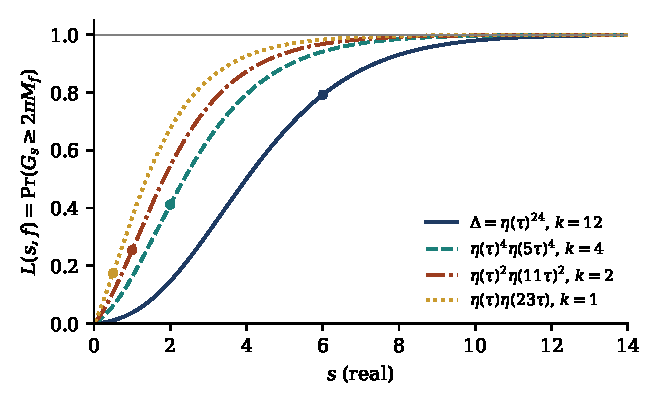
\includegraphics[width=\textwidth]{figs/ch11_lvalues.pdf}
\caption{$L(s,f)=\Prob(G_s\ge2\pi M_f)$ for real $s$, for the multiplicative eta products $\eta(\tau)^{24}$, $\eta(\tau)^4\eta(5\tau)^4$, $\eta(\tau)^2\eta(11\tau)^2$ and $\eta(\tau)\eta(23\tau)$, of weights $k=12,4,2,1$; $G_s$ is a gamma variable of shape $s$, independent of the extreme value $M_f$ of Theorem~\ref{thm:ch11general}. Each curve increases from $0$ to $1$; dots mark the central values $L(k/2,f)$.}
\label{fig:ch11lvalues}
\end{figure}

\section{Modularity as self similarity of the law}

At $\tau=iy$ the transformation $\Delta(-1/\tau)=\tau^{12}\Delta(\tau)$ reads $\Delta(i/y)=y^{12}\Delta(iy)$. In terms of $F$ it is a statement about the law of $M^*$.

\begin{proposition}[this book]\label{prop:ch11selfsim}
For all $y>0$,
\[
F(y)=y^{-12}\,e^{2\pi(y-1/y)}\,F(1/y).
\]
Consequently $F(y)\sim y^{-12}e^{-2\pi/y}$ as $y\to0$, and $1-F(y)\sim24e^{-2\pi y}$ as $y\to\infty$.
\end{proposition}

\begin{proof}
Inserting~\eqref{eq:ch11DeltaF} into $\Delta(i/y)=y^{12}\Delta(iy)$ gives
\[
e^{-2\pi/y}F(1/y)=y^{12}e^{-2\pi y}F(y),
\]
which rearranges to the identity (equivalently, raise~\eqref{eq:ch11Pmod} to the power $24$). The left tail follows from $F(1/y)\to1$, the right tail from $1-P^{24}\sim24(1-P)$.
\end{proof}

We checked the identity at $y=0.5,0.8,1.3$ to fifteen digits. So the law of $M^*$ on $(0,1)$ is determined by its law on $(1,\infty)$, and modularity exchanges the two tails: $\Prob(1/M^*\ge x)\sim x^{12}e^{-2\pi x}$ is a gamma tail of shape $13$, while $1-F(y)\sim24e^{-2\pi y}$ is the exponential tail of the $24$ slowest clocks, those with $n=1$.

The functional equation $\Lambda(s,\Delta)=\Lambda(12-s,\Delta)$ is an integrated form of this self similarity. A sharper reading recovers the P\'olya kernel $\Phi_\Delta$ of Chapter~\ref{ch:10} as a conditional law. Put $V_s=G_s/2\pi$.\index{P\'olya kernel}

\begin{proposition}[this book]\label{prop:ch11posterior}
Let $W=\log(G_6/2\pi)$ with $G_6$ independent of $M^*$. Conditionally on $\{G_6\ge2\pi M^*\}$, $W$ has density $\Phi_\Delta$, and for every complex $z$
\[
\Lambda(6+z,\Delta)/\Lambda(6,\Delta)=\E\bigl[e^{zW}\bigm| G_6\ge2\pi M^*\bigr].
\]
\end{proposition}

\begin{proof}
Let $g_6(y)=(2\pi)^6y^5e^{-2\pi y}/120$ be the density of $V_6$. For bounded measurable $h$,
\[
\E\bigl[h(V_6)1\{M^*\le V_6\}\bigr]=\int_0^\infty hFg_6\,dy=\frac{(2\pi)^6}{120}\int_0^\infty h(y)y^5\Delta(iy)\,dy .
\]
Extend to $h(y)=y^z$ by dominated convergence, using the bounds in Step 1 of the proof of Theorem~\ref{thm:ch11main}, and divide by the case $z=0$.
\end{proof}

In Bayesian terms $\Phi_\Delta$ is a posterior: a log gamma prior of shape $6$ on $W$, likelihood $F(e^W)$, and by self similarity a posterior symmetric about $0$, with variance $0.1123518$ as in Chapter~\ref{ch:10}.

\section{Multiplicative eta products}

Let $r_m\ge0$ be integers with $\sum_mm\,r_m=24$, and put
\[
f(\tau)=\prod_m\eta(m\tau)^{r_m}=q\prod_m\prod_{n\ge1}(1-q^{mn})^{r_m}=\sum_{n\ge1}a_nq^n,
\]
of weight $k=\frac12\sum_mr_m$. Dummit, Kisilevsky and McKay \cite{dkm1985}\index{eta product} determined which have multiplicative coefficients; our search over all $1575$ partitions of $24$ (testing $a_{mn}=a_ma_n$ for coprime $m,n$ with $mn\le300$) finds the same thirty: twenty eight of integral weight $1$ to $12$, and $\eta(8\tau)^3$, $\eta(24\tau)$ of weights $\frac32$, $\frac12$. Each is a holomorphic modular form for a congruence subgroup \cite{koehler2011}. The theorem below needs only that $L(s,f)=\sum a_nn^{-s}$ converges absolutely in a right half plane, and its proof checks this directly for every eta product. Let
\[
M_f=\max_m\max_{j\le r_m}\max_{n\ge1}\frac{E_{m,j,n}}{2\pi mn},\qquad F_f(y)=\Prob(M_f\le y)=\prod_mP(my)^{r_m},
\]
the maximum of $r_m$ independent copies of $M/m$ for each $m$.

\begin{theorem}[this book]\label{thm:ch11general}
Let $f=\prod_m\eta(m\tau)^{r_m}$ with $r_m\ge0$ and $\sum_mm\,r_m=24$. Then $f(iy)=e^{-2\pi y}F_f(y)$ for $y>0$, $L(s,f)$ continues to an entire function, and for every complex $s$
\[
L(s,f)=\E\bigl[Q(s,2\pi M_f)\bigr].
\]
For real $s>0$, $L(s,f)=\Prob(G_s\ge2\pi M_f)$; in particular $0<L(s,f)<1$, and $L(s,f)$ increases strictly to $1$ as $s\to\infty$.
\end{theorem}

\begin{proof}
Since $\eta(imy)=e^{-\pi my/12}P(my)$ and $\sum_mmr_m=24$, we get $f(iy)=e^{-2\pi y}F_f(y)$. Next, $(\operatorname{Im}\tau)^6|\Delta(\tau)|$ is invariant under $\SL_2(\Z)$ and tends to $0$ at the cusp, so it is bounded, and $|\eta(\tau)|\le C(\operatorname{Im}\tau)^{-1/4}$. Hence $|f(x+iy)|\le C_fy^{-k/2}$, and $a_n=e^{2\pi ny}\int_0^1f(x+iy)e^{-2\pi inx}\,dx$ at $y=1/n$ gives $|a_n|\le e^{2\pi}C_fn^{k/2}$. So $L(s,f)$ converges absolutely for $\operatorname{Re}s>k/2+1$, where termwise integration gives $(2\pi)^{-s}\Gamma(s)L(s,f)=\int_0^\infty f(iy)y^{s-1}\,dy$. By~\eqref{eq:ch11Pmod}, $P(x)\le e^{\pi/12}x^{-1/2}e^{-\pi/(12x)}$ for $x\le1$, so $F_f(y)\le Cy^{-k}e^{-c/y}$ for small $y$, with $c=\frac{\pi}{12}\sum_mr_m/m>0$. These two facts replace the appeal to Chapter~\ref{ch:02} and Step~1 in the proof of Theorem~\ref{thm:ch11main}. Since $F_f$ has a positive derivative on $(0,\infty)$, the rest of that proof and the proofs of Corollaries~\ref{cor:ch11bounds} and~\ref{cor:ch11monotone} apply word for word.
\end{proof}

Multiplicativity is not used in the proof. It is what gives the left side an Euler product, and so what makes the right side arithmetic.

\subsection{An elliptic curve}

The product $\eta(\tau)^2\eta(11\tau)^2$ is the newform of weight $2$ and level $11$ attached by Eichler and Shimura \cite{eichler1954,shimura1971} to the elliptic curve $E=11a$, $y^2+y=x^3-x^2-10x-20$. Here $M_f$ is the maximum of two copies of $M$ and two copies of $M/11$, and since $Q(1,c)=e^{-c}$ the theorem at $s=1$ reads
\[
L(E,1)=\E\bigl[e^{-2\pi M_f}\bigr]=\Prob(E_0\ge2\pi M_f)=0.2538419\ldots,
\]
with $E_0$ a standard exponential independent of $M_f$. The value agrees with PARI/GP to sixteen digits, and $L(E,1)/\Omega_E=0.2000000$ with $\Omega_E=1.2692093$, the value $c_{11}/|E(\Q)_{\mathrm{tors}}|^2=5/25$ (Tamagawa number $5$ at $11$, torsion of order $5$) predicted by the Birch and Swinnerton Dyer formula \cite{bsd1965} with trivial Tate Shafarevich group.\index{Birch and Swinnerton Dyer conjecture}

The probability is positive, so the analytic rank is $0$, and hence the Mordell Weil rank is $0$ by Kolyvagin \cite{kolyvagin1988} with Gross and Zagier \cite{grosszagier1986}. But positivity is equally visible from the Mellin integral of $f(iy)>0$, so this adds interpretation, not information; the same holds for all eight weight two multiplicative eta products, of levels $11,14,15,20,24,27,32,36$.

\subsection{Higher weight, weight one and theta series}

For $\eta(\tau)^4\eta(5\tau)^4$, of weight $4$ and level $5$, $L(2,f)=0.4118613$ is the probability that $G_2\ge2\pi M_f$; Table~\ref{tab:ch11values} gives more.

The weight one product $\eta(\tau)\eta(23\tau)$ is classical. It is half the difference of the theta series of $x^2+xy+6y^2$ and $2x^2+xy+3y^2$, and its coefficient at a prime $p\ne23$ is $N_p-1$, with $N_p$ the number of roots of $x^3-x-1$ modulo $p$ (checked for $p<400$; Chapter~\ref{ch:lap} compares all prime powers below $2\cdot10^5$). By Hecke \cite{hecke1937} its $L$ function is the Artin $L$ function\index{Artin $L$ function} $L(s,\rho)=\zeta_{\Q(\theta)}(s)/\zeta(s)$ of the two dimensional representation of $S_3$ of Chapter~\ref{ch:03}, with $\theta=1.3247\ldots$ the real root of $x^3-x-1$. Theorem~\ref{thm:ch11general} says that this Artin $L$ function is an expectation,
\[
L(s,\rho)=\E\bigl[Q\bigl(s,2\pi\max(M,M'/23)\bigr)\bigr],
\]
with $M,M'$ independent copies of $M$. At $s=1$ the class number formula for $\Q(\theta)$ (signature $(1,1)$, class number $1$, regulator $\log\theta$) gives
\[
\Prob\bigl(E_0\ge2\pi\max(M,M'/23)\bigr)=\frac{2\pi\log\theta}{\sqrt{23}}=0.3684093\ldots,
\]
which we checked to sixteen digits. At the centre, $L(\frac12,\rho)=0.1740363$.

The two forms of half integral weight are theta series of Dirichlet characters,
\[
\eta(24\tau)=\sum_{n\ge1}\chi_{12}(n)q^{n^2},\qquad\eta(8\tau)^3=\sum_{n\ge1}\chi_{-4}(n)\,n\,q^{n^2},
\]
with Dirichlet series $L(2s,\chi_{12})$ and $L(2s-1,\chi_{-4})$; Chapter~\ref{ch:beta} builds the P\'olya kernels of $L(s,\chi_{12})$ and $L(s,\chi_{-4})$ from them. For independent copies $M_1,M_2,M_3$ of $M$,
\[
\frac\pi4=\Prob\Bigl(E_0\ge\frac\pi4\max_{j\le3}M_j\Bigr),\qquad \beta(2)=\Prob\Bigl(G_{3/2}\ge\frac\pi4\max_{j\le3}M_j\Bigr),
\]
where $\beta(2)=L(2,\chi_{-4})=0.9159656$ is Catalan's constant, and $L(1,\chi_{12})=\log(2+\sqrt3)/\sqrt3=\Prob(G_{1/2}\ge\pi M/12)=0.7603460$. All three were checked by quadrature to twelve digits.

\begin{table}[t]
\centering
\small
\begin{tabular}{@{}lrrlll@{}}
\toprule
$f$ & $N$ & $k$ & $L(\frac k2,f)$ & $L(\frac{k+1}2,f)$ & $L(k,f)$\\
\midrule
$\eta(\tau)^{24}$ & 1 & 12 & 0.7921228 & 0.8393455 & 0.9945437\\
$\eta(\tau)^8\eta(2\tau)^8$ & 2 & 8 & 0.6812925 & 0.7543068 & 0.9710803\\
$\eta(\tau)^6\eta(3\tau)^6$ & 3 & 6 & 0.5600387 & 0.6552302 & 0.9190337\\
$\eta(2\tau)^{12}$ & 4 & 6 & 0.7805377 & 0.8543050 & 0.9862573\\
$\eta(\tau)^4\eta(5\tau)^4$ & 5 & 4 & 0.4118613 & 0.5320174 & 0.7938049\\
$\eta(3\tau)^8$ & 9 & 4 & 0.7599657 & 0.8578161 & 0.9757577\\
$\eta(\tau)^3\eta(7\tau)^3$ & 7 & 3 & 0.3329818 & 0.4672118 & 0.6875637\\
$\eta(\tau)^2\eta(11\tau)^2$ & 11 & 2 & 0.2538419 & 0.4070039 & 0.5460480\\
$\eta(\tau)\eta(2\tau)\eta(7\tau)\eta(14\tau)$ & 14 & 2 & 0.3302237 & 0.5008415 & 0.6414713\\
$\eta(\tau)\eta(3\tau)\eta(5\tau)\eta(15\tau)$ & 15 & 2 & 0.3501508 & 0.5228611 & 0.6614752\\
$\eta(6\tau)^4$ & 36 & 2 & 0.7010911 & 0.8618161 & 0.9400130\\
$\eta(\tau)\eta(23\tau)$ & 23 & 1 & 0.1740363 & 0.3684093 & 0.3684093\\
$\eta(2\tau)\eta(22\tau)$ & 44 & 1 & 0.3157625 & 0.5772184 & 0.5772184\\
$\eta(12\tau)^2$ & 144 & 1 & 0.6120576 & 0.8706850 & 0.8706850\\
\bottomrule
\end{tabular}
\caption{$L(s,f)=\Prob(G_s\ge2\pi M_f)$ at $s=\frac k2,\frac{k+1}2,k$ for fourteen multiplicative eta products $f$ of level $N$ and weight $k$ (for $k=1$ the last two columns coincide), computed with PARI/GP (\texttt{lfunetaquo}) and confirmed by quadrature; the functional equation of each form was checked numerically.}
\label{tab:ch11values}
\end{table}

Every entry of Table~\ref{tab:ch11values} lies in $(0,1)$, and each row increases with $s$, as Theorem~\ref{thm:ch11general} requires. Within each weight the values grow with the level: the clocks of $\eta(m\tau)$ ring at rates $2\pi mn$, so large $m$ makes $M_f$ small and easy to beat.

\section{Zeros as a probabilistic statement}

If $\rho$ is a zero of $L(s,\Delta)$, Theorem~\ref{thm:ch11main} gives $\E[Q(\rho,2\pi M^*)]=0$. At the first zero $\rho=6+9.2223794\,i$ our quadrature of the left side has modulus below $10^{-15}$. At the trivial zeros $s=0,-1,-2,\ldots$, $Q(s,c)=0$ for \emph{every} $c>0$, so the integrand itself vanishes. The nontrivial zeros arise by cancellation. For fixed $c>0$, $s\mapsto Q(s,c)$ also has complex zeros. For $c=2\pi y$, with $y$ the $10\%$, $50\%$ and $90\%$ quantiles of $M^*$, the zeros of smallest positive imaginary part are near $5.293+6.081i$, $7.003+7.009i$ and $9.669+8.264i$, off the line $\operatorname{Re}s=6$; the zeros of $L(s,\Delta)$ appear only after averaging. The Riemann hypothesis for $\Delta$ takes the following form, which is a reformulation, not progress.

\begin{conjecture}[Riemann hypothesis for $\Delta$, extreme value form]\label{conj:ch11rh}
If $0<\operatorname{Re}s<12$ and $\E[Q(s,2\pi M^*)]=0$, then $\operatorname{Re}s=6$.
\end{conjecture}

Hecke's formula
\[
\Lambda(s,\Delta)=\sum_{n\ge1}\tau(n)\bigl[\Gamma(s,2\pi n)(2\pi n)^{-s}+\Gamma(12-s,2\pi n)(2\pi n)^{s-12}\bigr],
\]
obtained by splitting the Mellin integral at $y=1$ and applying modularity on $(0,1)$, is also an incomplete gamma expansion, but its terms carry the signs of $\tau(n)$; ours averages one kernel against a probability law. For Riemann's $\xi$ the analogous probabilistic formula is $2\xi(s)=\E[Y^s]$ of Biane, Pitman and Yor \cite{bpy2001}, with $Y$ a constant multiple of the maximum of a Brownian excursion (Chapter~\ref{ch:10}). Proposition~\ref{prop:ch11posterior} gives $\Lambda(s,\Delta)$ a probabilistic reading of the same kind, and on the reciprocal side $\xi(\frac12)/\xi(\frac12+\sqrt s)$ is the Laplace transform of a generalized gamma convolution if and only if the Riemann hypothesis holds (Polson~\cite{polson2017}; Theorem~\ref{thm:10bmain}).

Why does this not prove the Riemann hypothesis? First, positivity of a mixing law controls the transform on the real axis (Corollary~\ref{cor:ch11monotone}), not the cancellation that creates zeros. Second, Theorem~\ref{thm:ch11general} holds for every eta product with $\sum mr_m=24$, multiplicative or not, so it does not see the Euler product, and without an Euler product zeros can leave the line, as Davenport and Heilbronn showed \cite{davenportheilbronn1936}. Third, the known sufficient conditions for a Fourier transform to have only real zeros \cite{polya1926,debruijn1950,newman1976} rest on special structure of the kernel (an explicit form in the theorems of P\'olya and de Bruijn, the Lee Yang property in Newman's), and nothing we have shown about $M^*$ supplies such structure. What the representation does provide is an exact probabilistic formula and an unbiased estimator of $L$ at complex points, though one whose variance grows exponentially with the height, as the next section shows.

\section{Monte Carlo}

Theorem~\ref{thm:ch11main} turns evaluation of $L(s,\Delta)$ into sampling. We truncate the maximum at $n\le N$ and call the result $M^*_N\le M^*$. Since $M^*_N\ne M^*$ requires some clock with $n>N$ to ring after $M^*_N$, the union bound gives
\[
\Prob\bigl(M^*>y\ge M^*_N\bigr)\le24\sum_{n>N}e^{-2\pi ny}=\frac{24\,e^{-2\pi(N+1)y}}{1-e^{-2\pi y}} .
\]
For real $s>0$ the bias is $\Prob(M^*_N\le V_s<M^*)$, at most the integral of the smaller of $1$ and this bound against the density of $V_s$, which for $s=6$ and $N=400$ is $1.2\times10^{-13}$. The algorithm draws $E_{j,n}$ for $j\le24$, $n\le N$, sets $m_r=\max_{j,n}E_{j,n}/(2\pi n)$, and returns the mean and standard error of $Q(s,2\pi m_r)$ over $R$ draws. With $N=400$ and $R=20000$ draws we obtained $0.7929\pm0.0012$ (one standard error) for $L(6,\Delta)=0.7921$. The empirical $10\%$, $50\%$, $90\%$ quantiles of $M^*$ were $0.394$, $0.569$, $0.869$, against exact values $0.3935$, $0.5708$, $0.8650$. For real $s>0$ the estimator is the conditional expectation of $1\{G_s\ge2\pi M^*_N\}$ given $M^*_N$, so by the Rao Blackwell theorem its variance is smaller, in our runs by a factor of about five. For a fixed sample, $s\mapsto R^{-1}\sum_rQ(s,2\pi m_r)$ is an entire empirical $L$ function. On the critical line, however, the summands are large while $L$ is not: for fixed $c$, $|Q(6+it,c)|\sim c^6e^{-c}e^{\pi t/2}/(\sqrt{2\pi}\,t^{13/2})$ as $t\to\infty$, because $1/|\Gamma(6+it)|$ grows like $e^{\pi t/2}$, and the standard deviation of $Q(6+it,2\pi M^*)$, computed by quadrature, is $0.18$ at $t=0$, $22$ at the first zero $t=9.22$ and $4.0\times10^6$ at $t=20$. Locating zeros by simulation therefore requires a cancellation that grows exponentially with the height.

\section{Hitting times}

If coupon $(j,n)$ is collected at time $E_{j,n}/(2\pi n)$, the number of coupons still missing at time $t>0$ is finite, with mean $24\sum_ne^{-2\pi nt}$. So $M^*$ is the time at which a collection that starts with infinitely many missing coupons is completed: the hitting time\index{hitting time} of the empty set by the decreasing Markov process of missing coupons, which enters from an infinite configuration. For real $s>0$, $L(s,\Delta)$ is the probability that the collection is completed before an independent gamma clock of shape $s$ and rate $2\pi$ rings.

The laws that Biane, Pitman and Yor \cite{bpy2001} build from theta functions are laws of Brownian functionals. Is $M$ a Brownian functional? We do not know, but a related identity holds. Let $K=\sup_{t\le1}|b_t|$ for a standard Brownian bridge $b$, so that $\Prob(K\le x)=\sum_{n\in\Z}(-1)^ne^{-2n^2x^2}$ is Kolmogorov's law \cite{kolmogorov1933}.

\begin{proposition}[this book]\label{prop:ch11kolmogorov}
$K^2$ has the law of the maximum of independent exponential variables, one of rate $2j$ for each even $j\ge2$ and two of rate $2j$ for each odd $j\ge1$. With $M_1,M_2,M_3$ independent copies of $M$, and $K$ independent of $M_3$,
\[
\max(M_1,M_2)\overset{d}{=}\max\bigl(K^2/\pi,\,M_3/2\bigr).
\]
\end{proposition}

\begin{proof}
Jacobi's triple product gives
\[
\sum_{n\in\Z}(-1)^nq^{n^2}=\prod_{n\ge1}(1-q^{2n})(1-q^{2n-1})^2.
\]
With $q=e^{-2x^2}$ the left side is $\Prob(K^2\le x^2)$ and each factor $1-q^j$ is the probability that an exponential variable of rate $2j$ is at most $x^2$; independence gives the first claim. The same identity in the form $\sum_n(-1)^nq^{n^2}=\eta(\tau)^2/\eta(2\tau)$, at $q=e^{-2\pi y}$, reads $P(y)^2=\Prob(K^2\le\pi y)\,P(2y)$, which is the second claim.
\end{proof}

We checked it at $y=0.1,0.2,0.5$ to fifteen digits. It suggests, but does not establish, that $M$ can be realised through passage or exit times of a diffusion. The simplest mechanism is excluded: the passage time of a one dimensional diffusion from an entrance or reflecting boundary to a fixed level is a sum of independent exponential variables \cite{kent1980}, and $M$ is not (Exercise~\ref{ex:ch11laplace}).

\begin{problem}\label{prob:ch11brownian}
Find a natural Brownian or Bessel functional with the law of $M$, or of $M^*$, or show that none exists among first passage and last exit times of one dimensional diffusions.
\end{problem}

\section{Notes}

That $\prod_n(1-e^{-2\pi ny})$ is a distribution function is elementary, and such products pervade the probabilistic literature on theta functions, from Kolmogorov \cite{kolmogorov1933} to Biane, Pitman and Yor \cite{bpy2001}. What we have not seen before is the representation of $L$ functions of eta products as expectations of incomplete gamma functions at an extreme value, with its consequences: special values as probabilities, monotonicity, modular self similarity, and the posterior reading of the P\'olya kernel. These are the results we label as ours.

Martin \cite{martin1996} classified the multiplicative eta quotients; for quotients our argument fails, since $1/(1-e^{-2\pi ny})$ is not a probability. K\"ohler \cite{koehler2011} is the reference for eta products and theta series, Gumbel \cite{gumbel1958} for extreme values, and Thorin \cite{thorin1977} and Bondesson \cite{bondesson1992} for gamma convolutions. Hecke's formula underlies the evaluation of $L$ functions in PARI/GP and the LMFDB \cite{lmfdb}.

\section{Exercises}

\begin{enumerate}
\item\label{ex:ch11mean} Prove $\E[M]=2/\sqrt3-3/\pi$. (Integrate the pentagonal series for $1-P(y)$ termwise, pair $k$ with $-k$, and evaluate $\int_0^1x(1-x^2)/(1+x^3)\,dx=2\pi/(3\sqrt3)-1$.)

\item Using $\Prob(aG_s<E)=\E[e^{-aG_s}]=(1+a)^{-s}$ for a standard exponential $E$ independent of $G_s$, and a union bound, prove for real $s>1$ that $1-L(s,f)\le\sum_mr_m\sum_{n\ge1}(1+mn)^{-s}$. Evaluate the bound for $\Delta$ at $s=12$ and compare with $1-L(12,\Delta)=0.0054563$.

\item Show that $M^*$ has density $2\pi(1-E_2(iy))F(y)$. Use the transformation law $E_2(-1/\tau)=\tau^2E_2(\tau)+6\tau/(\pi i)$ and Proposition~\ref{prop:ch11selfsim} to find its behaviour as $y\to0$.

\item Prove $\E[K^2]=\pi^2/12$ from Kolmogorov's series. Deduce from Proposition~\ref{prop:ch11kolmogorov} that $\E[\max(M_1,M_2)]\le\pi/12+\E[M]/2$, and check it numerically.

\item For real $s\in(0,12)$ let $W_s$ be $\log(G_s/2\pi)$ conditioned on $\{G_s\ge2\pi M^*\}$. Show that $\E[e^{zW_s}]=\Lambda(s+z,\Delta)/\Lambda(s,\Delta)$, that the law of $W_s$ is the exponential tilt of the law of $W_6$ by $e^{(s-6)u}$, and that $W_{12-s}\overset{d}{=}-W_s$.

\item\label{ex:ch11laplace} Show that $\E[e^{-uM}]=\sum_{k\in\Z}(-1)^ku/(u+\pi k(3k-1))$ for $\operatorname{Re}u>0$, and, using $\sum_{k\in\Z}(-1)^k/(k-a)=-\pi/\sin\pi a$, that with $w=\sqrt{1-12u/\pi}$
\[
\E\bigl[e^{-uM}\bigr]=\frac uw\Bigl(\csc\frac{\pi(1-w)}6-\csc\frac{\pi(1+w)}6\Bigr).
\]
Deduce that the meromorphic continuation of $\E[e^{-uM}]$ vanishes at $u=-35\pi/12$, and conclude that $M$ is not a sum of independent exponential variables. (The Laplace transform of $\sum_jE_j/\lambda_j$ is the reciprocal of the entire function $\prod_j(1+u/\lambda_j)$.)
\end{enumerate}

\section{Open computational problems}

\begin{compproblem}[Tables of the laws $M_f$]
Objective: reference tables of the laws $M_f$ for all thirty multiplicative eta products. Objects and scale: $F_f(y)=\prod_mP(my)^{r_m}$, densities, quantiles at levels $10^{-6},\ldots,1-10^{-6}$, means, variances and the first twenty negative moments, to $50$ digits. Route: the pentagonal series for $my\ge1$ and~\eqref{eq:ch11Pmod} above, in PARI/GP or mpmath; Newton iteration for quantiles. Deliverable: tables and a common plot of all thirty laws. Why it matters: these laws are the arithmetic content of Theorem~\ref{thm:ch11general}, and their tails encode weight and level through self similarity.
\end{compproblem}

\begin{compproblem}[Variance reduction and zero location]
Objective: make $\E[Q(s,2\pi M_f)]$ a practical estimator of $L(s,f)$ on the critical line. For $\Delta$ at $s=6+it$ the plain estimator has standard deviation $0.18$ at $t=0$, $22$ at the first zero and $4.0\times10^6$ at $t=20$, growing like $e^{\pi t/2}t^{-13/2}$. Objects and scale: $\Delta$ on $s=6+it$ and $\eta(\tau)^2\eta(11\tau)^2$ on $s=1+it$ for $0\le t\le30$, with up to $10^9$ draws. Route: GPU sampling of truncated maxima; control variates from the slowest clocks, which have equal rates (the $24$ clocks of rate $2\pi$ for $\Delta$, the two of rate $2\pi$ for the level $11$ form), so that their maximum has R\'enyi's representation, and from the exact values on the real axis; stratification on quantiles of $M_f$; randomised quasi Monte Carlo through the inverse distribution function. Deliverable: for each method the variance as a function of $t$ and its exponential rate, and the largest height up to which the zeros of the sample average locate the zeros of $L(s,f)$ to within $0.01$, with error bars. Why it matters: an estimator able to locate zeros would give a probabilistic certificate of their positions, independent of the approximate functional equation, and the growth rate measures the cancellation that any probabilistic route to the zeros must overcome.
\end{compproblem}

\begin{compproblem}[Eigenforms that are not eta products]
Objective: extend the representation to Hecke eigenforms $f$ for which $g_f(y)=e^{2\pi y}f(iy)$ is not a distribution function; when the root number is $-1$, $f(iy)$ changes sign. Since $g_f$ is smooth and of bounded variation, with $g_f(0+)=0$ and $g_f(\infty)=1$, its Jordan decomposition gives $g_f=aF_1-bF_2$ with distribution functions $F_1,F_2$ on $(0,\infty)$, $a-b=1$, and $a+b$ equal to the total variation $V_f$ of $g_f$, the least possible value; the proof of Theorem~\ref{thm:ch11general} then gives $L(s,f)=a\E[Q(s,2\pi X_1)]-b\E[Q(s,2\pi X_2)]$ with $X_i$ of law $F_i$. Objects and scale: all newforms of weight $2$ with rational coefficients and level up to $500$, and the level one eigenforms of weights $16$ to $24$. Route: $q$ expansions from PARI/GP \texttt{mfinit} or the LMFDB, with the Fricke involution for small $y$; $V_f$ by quadrature of $|g_f'|$; linear programming over mixtures of the laws $\prod_mP(my)^{r_m}$ and their rescalings, to approximate $F_1$ and $F_2$ by extreme value laws. Deliverable: for each form $V_f$ and $b=(V_f-1)/2$, against level, weight, root number and rank, and the error of the best extreme value approximations. Why it matters: $b$ measures the distance from the positive world of this chapter; it is positive whenever $L(\frac k2,f)=0$, in particular for every elliptic curve of positive rank, since then $L(1,f)=0$ by Kolyvagin's theorem \cite{kolyvagin1988}.
\end{compproblem}

